\documentclass[tikz, margin=3mm]{standalone}
\usepackage{tikz}

\begin{document}
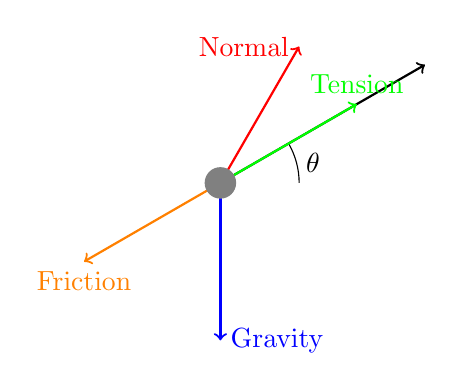
\begin{tikzpicture}

    % Define the angle of slope
    \pgfmathsetmacro{\angle}{30}
    
    % Draw the slope
    \draw[thick, ->] (0,0) -- (\angle:3cm);
    \draw (1cm,0) arc (0:\angle:1cm) node[midway, right] {$\theta$};
    
    % Draw Forces
    \draw[thick, ->, red] (0,0) -- ++(90-\angle:2cm) node[left] {Normal};
    \draw[thick, ->, blue] (0,0) -- ++(-90:2cm) node[right] {Gravity};
    \draw[thick, ->, green] (0,0) -- ++(\angle:2cm) node[above] {Tension};
    \draw[thick, ->, orange] (0,0) -- ++(180+\angle:2cm) node[below] {Friction};
    
    % Draw the box
    \fill[gray] (0,0) circle (2mm);
    
\end{tikzpicture}
\end{document}